\chapter*{Introduction}
\begin{figure}[h]
	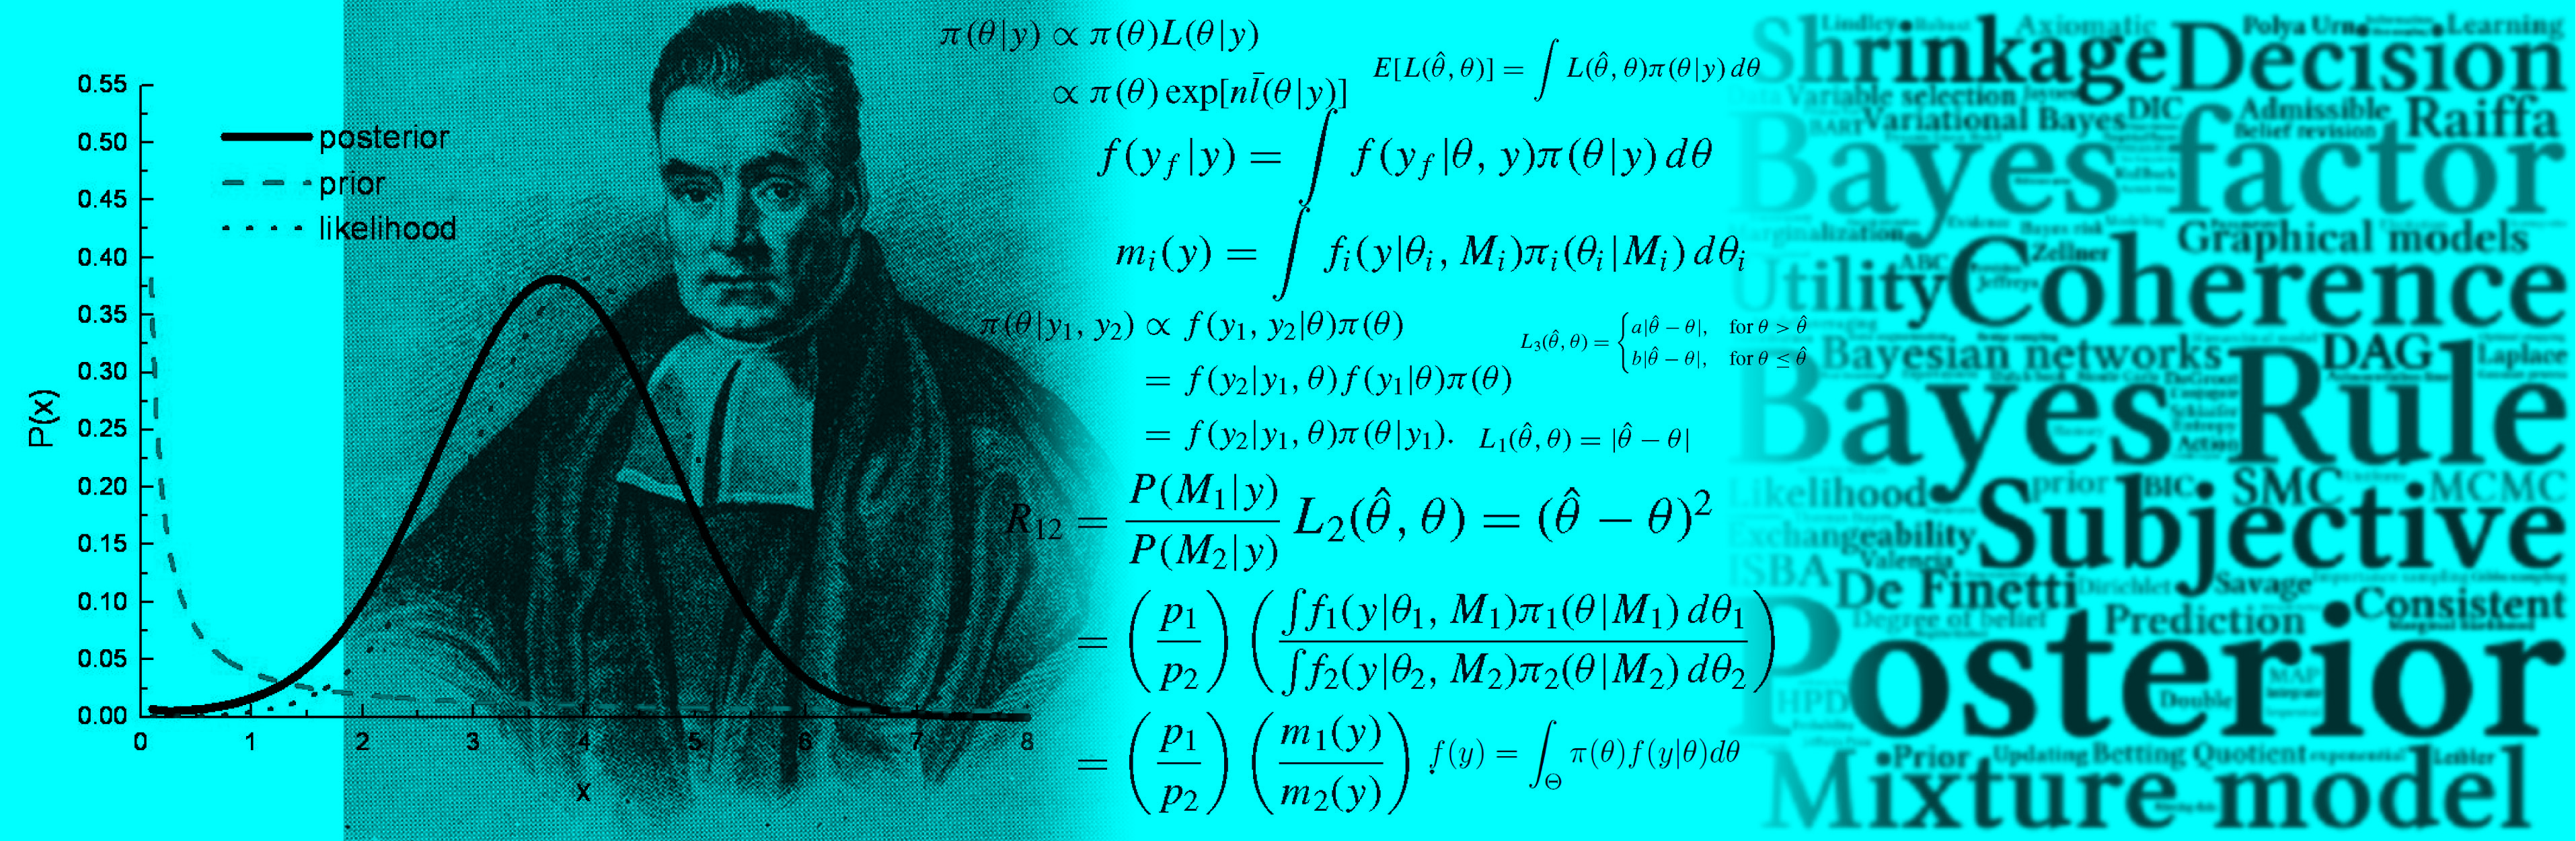
\includegraphics[width=340pt, height=150pt]{frontmatter/figures/BannerBook.jpg}
	%%\centerline{\epsfig{/Chapters/chapter1/figures/cat.eps,width=.8\textheight,height=.4\textwidth}}
	\caption[List of figure caption goes here]{\textit{Supposedly} portrait of Thomas Bayes.}\label{fig01}
\end{figure}

Since the late 90s, Bayesian inference has gained significant popularity among researchers due to the computational revolution and the availability of algorithms to solve complex integrals. However, many researchers, students, and practitioners still lack a deep understanding and practical application of this inferential approach. The primary reason for this is the requirement for strong programming skills.


\textbf{Introduction to Bayesian Econometrics: A GUIded Toolkit using R} mainly targets those who want to apply Bayesian inference with a good conceptual and formal understanding, but who may not necessarily have the time to develop programming skills. Thus, this book provides a graphical user interface (GUI) to carry out Bayesian regression in a very user-friendly environment. The book also offers the basic theory and its code implementation using \textbf{R} software \cite{R2021}, along with some applications to highlight the potential of Bayesian inference. Additionally, it includes theory and computational exercises for those interested in developing more complex models. In particular, this book presents the mathematical proofs of the basic models step-by-step in the first part, which serve as the foundation for obtaining the most relevant mathematical results in the more complex models covered in the second and third parts.

Our GUI is based on an interactive web application using \texttt{shiny} \cite{Chang2018}, along with several packages in \textbf{R}. Users can estimate univariate, multivariate, time series, longitudinal/panel data, and Bayesian model averaging models using our GUI. In addition, it provides basic summaries, as well as formal and graphical diagnostics of the posterior chains. Our GUI can be run on any operating system and is freely available at \textbf{https://github.com/besmarter/BSTApp}.

Users can access simulated and real datasets in the folders \textbf{DataSim} and \textbf{DataApp}, respectively. The former folder also includes the files used to simulate different processes, so the population parameters are available. As a result, these files can be used as a pedagogical tool to demonstrate various statistical properties. The latter folder contains the datasets used in our applications. Users are encouraged to use these datasets as templates for structuring their own datasets.

This book is divided into three parts. The first part covers the theory (both conceptual and mathematical), programming, and simulation foundations (chapters 1 to 4). The second part focuses on the applications of regression analysis, with particular emphasis on the computational aspect of obtaining draws from the posterior distributions at three levels of programming skills: no skills at all using our GUI, intermediate skills using specialized \textbf{R} packages for Bayesian inference, and relatively advanced programming skills to obtain posterior draws from scratch (chapters 5 to 10). The third part provides an introductory treatment of \textit{advanced methods} in Bayesian inference (chapters 11 to 14). 

I present some of the mathematical deductions in detail in the first part of the book, whereas I do not show most of the proofs in the second and third parts. However, the same mathematical steps in the first part can be used to derive the results in parts two and three.

In the first part, Chapter \ref{chap1} begins with an introduction to formal concepts in Bayesian inference, starting with Bayes' rule, its components, their formal definitions, and basic examples. It then presents the basics of Bayesian inference based on decision theory under uncertainty. Chapter \ref{chap2} discusses the conceptual differences between Bayesian and Frequentist statistical approaches, as well as provides a historical and philosophical perspective on Bayesian statistics and econometrics, highlighting the contrasts with the Frequentist approach. In Chapter \ref{chap4}, I introduce conjugate families in basic statistical models, solving them both analytically and computationally. Simulation-based methods are presented in Chapter \ref{chap5}; these algorithms are crucial in modern Bayesian inference since most realistic models do not have standard forms or analytical solutions. 

In the second part, Chapter \ref{chapGUI} presents our graphical user interface, and univariate and multivariate regression models are covered in Chapters \ref{chap6} and \ref{chap7}. Chapter \ref{chap8} focuses on univariate and multivariate time series models, while Chapter \ref{chap9} covers Bayesian longitudinal/panel data models. Chapter \ref{chap10} introduces Bayesian model averaging. In the third part, Chapter \ref{chap11} explores semi-parametric and non-parametric models, Chapter \ref{chap13} covers Bayesian methods in machine learning algorithms, Chapter \ref{chap12} discusses causal inference, and Chapter \ref{chap15} describes approximation methods.

\textbf{About me}\\
My name is Andrés Ramírez-Hassan, and I am an applied and theoretical econometrician working as a Distinguished Professor in the School of Finance, Economics, and Government at Universidad EAFIT (Medellín, Colombia). I hold a PhD in Statistical Science, a Master's degree in Finance, another in Economics, and a Bachelor's degree in Economics. I was a research fellow at the Department of Econometrics and Business Statistics at Monash University, and a visiting Professor in the Department of Economics at the University of Melbourne and the University of Glasgow. 

Since completing my PhD, much of my research has focused on Bayesian Econometrics, with applications in crime, finance, health, sports, and utilities. My work has been published (or is forthcoming) in highly regarded journals such as the \textit{International Journal of Forecasting}, \textit{Journal of Applied Econometrics}, \textit{Econometric Reviews}, \textit{Journal of Computational and Graphical Statistics}, \textit{The R Journal}, \textit{Economic Modelling}, \textit{Spatial Economic Analysis}, \textit{Economic Inquiry}, \textit{World Development}, \textit{Journal of Sport Economics}, \textit{Empirical Economics}, \textit{Australian and New Zealand Journal of Statistics}, \textit{Brazilian Journal of Probability and Statistics}, and other prestigious international research outlets.

I founded \textbf{BEsmarter} -- \textbf{B}ayesian \textbf{E}conometrics: \textbf{s}imulations, \textbf{m}odels, and \textbf{a}pplications to \textbf{r}esearch, \textbf{t}eaching, and \textbf{e}ncoding with \textbf{r}esponsibility. This is a research group whose \textbf{mission} is to \textit{lead and excel in the generation and dissemination of Bayesian Econometric knowledge through research, teaching, and software}. We \textbf{envision} \textit{worldwide econometric research, teaching, and applications based on the Bayesian framework that:}

\begin{itemize}
	\item Inspires new econometric ideas,
	\item Creates a user-friendly environment for applications of Bayesian econometrics,
	\item Transforms classic econometric research, teaching, and applications, 
	\item where one of the main concerns of science is to solve social problems.  
\end{itemize}

\textbf{Contact:} aramir21@gmail.com / aramir21@eafit.edu.co

\textbf{Website:} \textbf{http://www.besmarter-team.org}\\
%\textbf{https://sites.google.com/view/arh-bayesian}

\begin{figure}[h]
	
\includegraphics[width=80pt, height=20pt]{frontmatter/figures/by-nc-sa.png}
	%%\centerline{\epsfig{/Chapters/chapter1/figures/cat.eps,width=.8\textheight,height=.4\textwidth}}
	\caption[List of figure caption goes here]{This book is licensed under the \textbf{Creative Commons Attribution-NonCommercial-ShareAlike 4.0 International License}.}\label{fig02}
\end{figure}




